\section{Analysis of the Maximum Clique Cover Algorithm}\label{sec:naive}
In this section we will prove Theorem~\ref{thm:naive}.
Specifically, we want to show that the event,
\[
\text{a size-$d$ clique $\he$ appear in $\pG$ but is not a hyperedge in $\rhG$},
\]
happens with probability $o_n(1)$ when $\delta<\frac{d-3}{d}$ but happens with at least constant probability when $\delta\ge \frac{d-3}{d}$.

Let us prove the two claims respectively in the following two lemmas. 

\begin{figure}[ht]
\centering
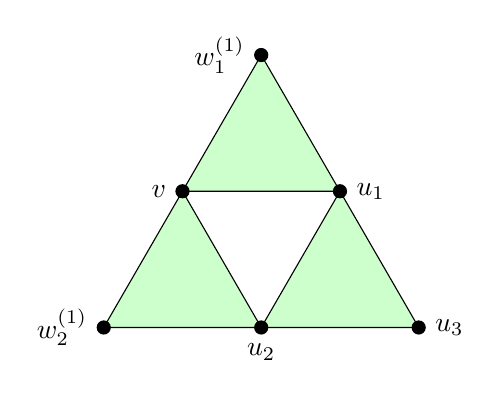
\begin{tikzpicture}
% Define vertices
\coordinate (A) at (0,0);
\coordinate (B) at (2,0);
\coordinate (C) at (1,1.73);
\coordinate (D) at (-1,-1.73);
\coordinate (E) at (1,-1.73);
\coordinate (F) at (3,-1.73);  % 1.73 approximates sqrt(3), for equilateral triangles
% Draw triangles
\fill[fill=green!20] (A)--(B)--(C);
\fill[fill=green!20] (B)--(E)--(F);
\fill[fill=green!20] (A)--(D)--(E);


% Draw nodes on top of filled triangles
\node[draw, circle, scale=0.5, fill=black, label=left:$v$] at (A) {};
\node[draw, circle, fill=black, scale=0.5, label=right:$u_1$] at (B) {};
\node[draw, circle, fill=black,  scale=0.5,label=left:$w_1^{(1)}$] at (C) {};
\node[draw, circle, fill=black,  scale=0.5,label=left:$w_2^{(1)}$] at (D) {};
\node[draw, circle, fill=black,  scale=0.5,label=below:$u_2$] at (E) {};
\node[draw, circle, fill=black, scale=0.5,label=right:$u_3$] at (F) {};

\draw (A)--(B)--(C)--cycle;
\draw (A)--(D)--(E)--cycle;
\draw (B)--(E)--(F)--cycle;
\end{tikzpicture}
\caption{Illustration of $\naH$ when $d=3$.}
\label{fig:fake-hyperedge}
\end{figure}

\begin{lemma}
    When $\delta\ge \frac{d-3}{d}$, 
    \[
    \Pr\B(\exists \he\in\binom{[n]}{d} \text{ s.t. } \he  \text{ is a clique in $\pG$ but } \he\notin \hE_\rhG\B)=\Omega_n(1)\,.
    \]
\end{lemma}
\begin{proof}
We will focus on a sufficient condition that $\he = \{v,u_1,\cdots,u_{d-1}\}$ is a clique but does not appear in  $\hE_\rhG$. Then we will use second moment method to lower bound the probability of that sufficient condition happening at one of the hyperedges. The sufficient condition is that $\he\notin \hE_\rhG$ and all of the following hyperedges are in $\hE_\rhG$:
\begin{itemize}
    \item $\{u_1,u_2,\cdots,u_d\}$ and
    \item $\{v,u_i,w_i^{(1)},\cdots, w_i^{(d-2)}\}$ for all $1\le i\le d-1$.
\end{itemize}
Let $\naH$ denote the hypergraph, see Figure~\ref{fig:fake-hyperedge} for an illustration (we abuse notation and let $\naH$ include the non-hyperedge $\he$).
There are $v_\naH=d^2-2d+3$ nodes  and $e_\naH=d$ edges in $\naH$. $p=n^{-d+1+\delta} =\Omega_n (n^{-d+2+3/d}) = \Omega_n (n^{-v_\naH/e_\naH})$.
Let $\naH_1,\naH_2,\cdots,\naH_t$ be all copies of such sub-hypergraph on the complete graph of $[n]$, we have
\[
t=\binom{n}{v_\naH}\frac{(v_\naH)!}{\aut(\naH)}=\Theta_n(n^{v_\naH})\,.
\]
Here $\aut(\naH)$ is the number of automorphisms of $\naH$.
Let $I_i$ be the indicator that $\naH_i$ is in $\rhG$. And $X_\naH = \sum_{i=1}^tI_i$ be the number of such event happening. We have
\[
\E [X_\naH] = tp^{e_\naH}(1-p) = \Theta_n(n^{v_\naH}p^{e_\naH})\,.
\]
And 
\[
\var(X_\naH) = \sum_{i=1}^t\sum_{j=1}^t \cov(I_iI_j) = 
\sum_{i=1}^t\sum_{j=1}^t (\Pr(I_i=I_j=1)-\Pr(I_i=1)\Pr(I_j=1))\,.
\]
We have $\Pr(I_i=1) = \Pr(I_j=1) = p^{d}(1-p)$. If the non-hyperedge in $\naH_i$ overlaps with a hyperedge in $\naH_j$ or vice versa, then $\cov(I_i,I_j)$ are negative. So to get an upper bound of $\var(X_\naH)$, we only consider pairs $(\naH_i,\naH_j)$ that are positively correlated. 
Consider pairs $(\naH_i,\naH_j)$ such that $\naH_i\cap \naH_j = K$, where $K\subset \naH$ is a sub-hypergraph of $\naH$ with non-empty edge set.
\begin{align*}
\var(X_\naH) &= O_n\B( \sum_{\substack{K \subseteq \naH,\\ e_K > 0}} n^{2v_\naH - v_K} \left( p^{2e_\naH - e_K} - p^{2e_\naH} \right) \B) \\
&= O_n\B( n^{2v_\naH} p^{2e_\naH} \sum_{\substack{K \subseteq H,\\ e_K > 0}} n^{-v_K} p^{-e_K} \B).
\end{align*}
Then from Lemma~\ref{lem:non-zero}, 
\[
\Pr(X_\naH\ne 0) \ge \frac{(\E X_\naH)^2}{(\E X_\naH)^2+\var(X_\naH)} = \frac{1}{1+O_n(\sum_{\substack{K\subseteq \naH,\\ e_K > 0}} n^{-v_K} p^{-e_K})}\,.
\]
We can easily check that for any $K\subset \naH$, $\frac{e_K}{v_K}\le \frac{e_\naH}{v_\naH}$. So by $p=\Omega_n (n^{-v_\naH/e_\naH})$, we have
\[
\sum_{\substack{K\subseteq \naH,\\ e_K > 0}} n^{-v_K} p^{-e_K} = \sum_{\substack{K\subseteq \naH,\\ e_K > 0}} O_n(n^{-v_\naH} n^{v_\naH }) = O_n(1)\,.
\]
This means $\Pr(X_\naH\ne 0) = \Omega_n(1)$.
\end{proof}
% For a specific choice of $d^2-2d+3$ vertices $V$: $v$, $\{u_i:1\le i\le d\}$ and $\{w_i^{(j)}:1\le i\le d-1,1\le j\le d-2\}$, let event 
% We introduce a definition of inclusion.
% \begin{definition}
%     We say an \emph{inclusion} happens at a size-$r$  set $S$ if $S$ is still a clique in the projected graph of $E\backslash \{S\}$.
% \end{definition}
% And the following holds.
% \[
% \begin{split}
% &\Pr([d] \text{ is a clique in $\pG$ but } [d]\notin \hE_\rhG)\\
% &= \Pr(\forall i,j\in [d],\exists \he\in \hE_\rhG, i,j\in \he|[d]\not\in \hE_\rhG)(1-p).
% \end{split}
% \]
% Let $\pinc$ denote $\Pr(\text{an inclusion happens at $[r]$})$.
% From the lemma below, \eqref{eq:clique-not-hedge} is $O(n^{-1/2})=o(1)$ as desired.

\begin{lemma}
When $\delta<\frac{d-3}{d}$,
\[
    % \Pr([d] \text{ is a clique in $\pG$ but } [d]\notin \hE_\rhG)= O_n(n^{\binom{d}{2}(-1+\delta)})
    % .
    \Pr\B(\exists \he\in\binom{[n]}{d} \text{ s.t. } \he  \text{ is a clique in $\pG$ but } \he\notin \hE_\rhG\B)=o_n(1)\,.
\]
\end{lemma}
By union bound over all possible cliques in $\binom{[n]}{d}$, the above probability is upperbounded by 
\[
\binom{n}{d}\Pr([d] \text{ is a clique in $\pG$ but } [d]\notin \hE_\rhG) = \binom{n}{d}(1-p)\Pr(\forall i,j\in [d],\exists \he\in \hE_\rhG, i,j\in \he\b|[d]\not\in \hE_\rhG)
\]

Now we split the event as follows. Let $\mathcal{S} = \{S_1,S_2,\cdots, S_{m}\}$ be all non-empty proper subsets of $[d]$ with size at least 2, $m=2^d-2-d$. Let $A_i$ be the event that at least one of edges in the set 
\[\hE_i=
\B\{\he\in \binom{[n]}{d}\B|\he\cap [d] = S_i\B\}
\]
is included in $\hE_\rhG$. Then the event that $[d]$ is a clique in $\pG$ but $[d]\notin \hE_\rhG$ is equivalent to the event that every pair $j,k\in[d]$ is included in some $S_i$ where $A_i$ happens. We have
\begin{align*}
&\  \Pr(\forall i,j\in [d],\exists \he\in \hE_\rhG, i,j\in \he\b|[d]\not\in \hE_\rhG) \\
&= \sum_{I\subset [m]} \1\{\forall j,k\in[r], \exists i\in I, j,k\in S_i\} \Pr((\cap_{i\in I}A_i)\cap(\cap_{i\in [m]\backslash [I]}A_i^c) )\\
&\le \sum_{I\subset [m]} \1\{\forall j,k\in[r], \exists i\in I, j,k\in S_i\} \Pr(\cap_{i\in I}A_i)\\
&= \sum_{I\subset [m]} \1\{\forall j,k\in[r], \exists i\in I, j,k\in S_i\} \prod_{i\in I}\Pr(A_i) \numberthis\label{eq:union-events}
.
\end{align*}
The last inequality is because $\hE_i$ are disjoint sets of edges, so $A_i$ are independent events. 

Note that there are $\binom{n}{d-|S_i|}$ edges in $\hE_i$, we have 
\[
\Pr(A_i)\le  1-(1-p)^{\binom{n}{d-|S_i|}}\le pn^{d-|S_i|}\le n^{-(|S_i|-1-\delta)}
.
\]
Since there are $O_n(1)$ terms in \eqref{eq:union-events}, we have
\[
\Pr(\forall i,j\in [d],\exists \he\in \hE_\rhG, i,j\in \he\b|[d]\not\in \hE_\rhG) = O_n\b(n^{-g_0(\delta)}\b).
\]
Recall that \[
g_0(\delta) = \min_{\substack{I\subset [m]:\\ \proj([d]) \subset \cup_i\proj(S_i)}} \sum_{i\in I}(|S_i|-1-\delta)\,.
\]
Therefore, 
\begin{equation*}
 \Pr\B(\exists \he\in\binom{[n]}{d} \text{ s.t. } \he  \text{ is a clique in $\pG$ but } \he\notin \hE_\rhG\B)  = O_n\b(n^{d-g_0(\delta)}\b)  \,.
\end{equation*}
The calculation of $g_0(\delta)$ is a nontrivial combinatorial optimization problem. 

Assuming Lemma~\ref{lem:optimal-clique-cover}, and note that $g_0(\delta)$ is strictly decreasing in $\delta$, we have for any $\delta<\frac{d-3}{d}$, $g_0(\delta)<d$. And thus 
\begin{equation*}
 \Pr\B(\exists \he\in\binom{[n]}{d} \text{ s.t. } \he  \text{ is a clique in $\pG$ but } \he\notin \hE_\rhG\B)  = O_n\b(n^{d-g_0(\delta)}\b)=o_n(1)  \,.
\end{equation*}

\begin{lemma}\label{lem:optimal-clique-cover}
Let $\cS = \{S_1,S_2,\cdots S_m\}$ be the set of all proper subsets of $[d]$ with size at least 2. When $\delta = \frac{d-3}{d}$, 
\[
g_0(\delta) =\min_{\substack{\cS'\subset \cS:\\ \proj([d]) \subset \proj(\cS')}} \sum_{S\in \cS'}(|S|-1-\delta)=d\,,
\]
achieved by the following set of subsets:
$\{2,3,\cdots,d\},\{1,2\},\{1,3\},\cdots,\{1,d\}$.
\end{lemma}
% The conjecture is verified by a computer for $d=3,4,5,6$.

\begin{proof}
    % \cg{cg: this can be proved with concavity when number of cliques is at least d and induction when size is at most d}
We will prove this under two separate cases. The first case is when $|\cS'|\ge d$, this is done by relaxation of the problem to real number. The second case is when $|\cS'|\le d$, which is done by induction on $d$.

\paragraph{Case 1: $|\cS'|\ge d$.}Let's begin with the first case. We will prove 
\[
f(\delta) =\min_{\substack{\cS'\subset \cS,|\cS'|\ge d:\\ \proj([d]) \subset \proj(\cS')}} \sum_{S\in \cS'}(|S|-1-\delta)=d\,.
\]
This part of the proof is similar to what we did in Lemma~\ref{lem:cover-bound}.
 % of $\{S_i\}_{i\in I}$, the union of edges is a superset of all edges in $\proj([d])$. 
We can get a lower bound on $f(\delta)$ by relaxing the set of possible $\cS'$ to be the set of cliques with at least $\binom{d}{2}$  number of edges. Also each clique in the set $\cS'$ that reaches minimum contains a unique edge, so $|\cS'|\le \binom{d}{2}$. We have
\[
f(\delta)\ge 
\min_{\substack{\cS'\subset \cS,d\le |\cS'|\le \binom{d}{2}:\\ \sum_{i\in I}\binom{|S_i|}{2} \ge \binom{d}{2} }} \sum_{i\in I}(|S_i|-1-\delta)
\,.
\]
Substituting $|S_i|$ with $x_i$ and relaxing it to real numbers, we get another lower bound on $f(\delta)$:
\[
\min_{M\in \mathbb{Z}^+,d\le M\le \binom{d}{2}}
\min_{\substack{x_1,x_2,\cdots, x_M\ge 2:\\ \sum_{i=1}^M\frac{x_i(x_i-1)}{2} \ge \binom{d}{2}} } \sum_{i=1}^M(x_i-1-\delta)
\,.
\]
% So 
% \[
% \begin{split}
% &\min_k \{g_k(\delta)+k-d\}\\
% &\ge 
% \min_{\substack{M\in \mathbb{Z}^+,\\ M\le \binom{d}{2}-1}}
% \min_{2\le k\le d}
% \min_{\substack{x_1,x_2,\cdots, x_M\ge 2:\\ \sum_{i=1}^M\frac{x_i(x_i-1)}{2} \ge \binom{d}{2}-\binom{k}{2}} } \B\{\sum_{i=1}^M(x_i-1-\delta)+k-d\B\}\\
% & = 
% \min_{\substack{M\in \mathbb{Z}^+,\\ M\le \binom{d}{2}-1}}
% \min_{\substack{x_0,x_1,\cdots, x_M\ge 2:\\ \sum_{i=0}^M\frac{x_i(x_i-1)}{2} \ge \binom{d}{2}} }\B\{ \sum_{i=0}^M x_i - M(1+\delta)-d\B\}\,.
% \end{split}
% \]
% Here in the equality we substituted $k$ with $x_0$.
By setting $y_i=\frac{x_i(x_i-1)}{2}$, the above can be written as 
\[
\min_{\substack{M\in \mathbb{Z}^+,\\d\le M\le \binom{d}{2}}}
\min_{\substack{y_1,\cdots, y_M\ge 1:\\ \sum_{i=0}^M y_i \ge \binom{d}{2}} }\B\{ \sum_{i=1}^M \B(\frac{1+\sqrt{1+8y_i}}{2}\B) - M(1+\delta)\B\}\,.
\]
For a fixed $M$, this is minimizing a concave function of $y$ over a polyhedron. So the minimum is either at a vertex or infinity. The later is obviously not the minimum. So the minimum is at a vertex of the following polyhedron:
\[
P= \B\{y:y_i\ge 1, \sum_{i=0}^M y_i \ge \binom{d}{2}\B\}\,.
\]
By symmetry of the function and $P$ under permutation of coordinates, we can consider one of the vertices without loss of generality. Let $y_1=y_2=\cdots=y_{M-1} = 1$, $y_M=\binom{d}{2}-M+1$, we have that the above is equal to
\[
\min_{\substack{M\in \mathbb{Z}^+,\\ 2\le M\le \binom{d}{2}}} \B\{ (M-1)(1-\delta)-1-\delta+  \frac{1+\sqrt{1+8(d(d-1)/2-M+1))}}{2}\B\}\,.
\]
The function is concave in $M$, so the minimum is at $M=2$ or $M=\binom{d}{2}$. When $\delta=\frac{d-3}{d}$ and $M=\binom{d}{2}$, the function is $3(d-1)/2>d$. When $\delta=\frac{d-3}{d}$ and $M=d$,  the function is $d$. So $f(\delta)\ge d$ when $\delta =\frac{d-3}{d} $
\paragraph{Case 2: $|\cS'|\le d$.} Next we prove the second case. We will show 
\[
h(d) \defeq\min_{\substack{\cS'\subset \cS,|\cS'|\le d:\\ \proj([d]) \subset \proj(\cS')}} \sum_{S\in \cS'}(|S|-1-\frac{d-3}{d})=d\,.
\]
Use induction on $d$. For $d=3$ there is only one possible $\cS'$, it's easy to verify that $h(3)=3$. 

Now assume $h(d-1) = d-1$, we want to show $h(d)=d$. For the simplicity of discussion, let $D(d)$ be the set of $\cS'$ that satisfy $|\cS'|\le d$ and $\proj([d]) \subset \proj(\cS')$. Also define a functional $F(\cS') \defeq \sum_{S\in \cS'}(|S|-1-\frac{d-3}{d})$. For any $\cS'\in D(d)$ and any $v\in[d]$, let us define a mapping $M_v(\cS'):D(d)\rightarrow D(d-1)\cup \{\bot\}$,
\[
M_v(\cS') = 
\begin{cases}
    \bot &\text{ if } ([d]\backslash\{v\})\in \cS'\\
    \{S\backslash\{v\}:S\in \cS', |S\backslash\{v\}|>1\} &\text{ otherwise } 
\end{cases}
\]
For now assume there exists a $v\in [d]$ that satisfy the two following properties,
\begin{itemize}
    \item $([d]\backslash\{v\})\not\in \cS'$ and
    \item $|\{S\in \cS': |S|=2,v\in S\}|\le 1$.
\end{itemize}
We will prove why such $v$ exists later. We have
\[
\begin{split}
&F(\cS')-F(M_v(\cS'))\\
&=\sum_{S\in \cS'}(|S|-1-\frac{d-3}{d}) - \sum_{S\in M_v(\cS')}(|S|-1-\frac{d-4}{d-1})\\
&=(\frac{d-4}{d-1}-\frac{d-3}{d})|\cS'|+\sum_{S\in \cS'}(|S|-1-\frac{d-4}{d-1})- \sum_{S\in M_v(\cS')}(|S|-1-\frac{d-4}{d-1})\\
&\ge -\frac{3}{d-1} +\sum_{S\in \cS',v\in S,|S|>2}1 +\sum_{S\in \cS',v\in S,|S|=2}(1-\frac{d-4}{d-1})\\
&= -\frac{3}{d-1} +\sum_{S\in \cS',v\in S}1 - \sum_{S\in \cS',v\in S,|S|=2}\frac{d-4}{d-1}\,.
\end{split}
\]
For the inequality, we used that $|\cS'|\le d$. By the assumption on $v$, we have $|S\in \cS',v\in S,|S|=2|\le 1$. Also $ v$ cannot only be contained in one set $S$ in $\cS'$, otherwise as for any vertex $u\ne v$, pair $\{v,u\}$ is contained in some set, $S$ would contain all nodes in $[d]$, contradicting the fact that $\cS$ only contain proper subsets of $[d]$. So $|S\in \cS',v\in S|\ge 2$. Taking all these into the inequality above, we have
\[
F(\cS')-F(M_v(\cS'))\ge  -\frac{3}{d-1}+2-\frac{d-4}{d-1} = 1\,.
\]
By induction assumption, $F(M_v(\cS'))\ge d-1$, so $F(\cS')\ge d$. This holds for any $\cS'\in D(d)$, so $h(d)\ge d$. As $d$ can be achieved by the configuration in the lemma statement, we have $h(d)=d$.

What remains is to show there exists $v$ that satisfy $([d]\backslash\{v\})\not\in \cS'$ and
 $|\{S\in \cS': |S|=2,v\in S\}|\le 1$. For contradiction suppose every $v$ either satisfy $([d]\backslash\{v\})\in \cS'$ or $|\{S\in \cS': |S|=2,v\in S\}|\ge 2$. Suppose there are $s$ nodes in $[d]$ satisfy $|\{S\in \cS': |S|=2,v\in S\}|\ge 2$, denote this set of nodes by $T$, and at least $d-s$ nodes satisfy $([d]\backslash\{v\})\in \cS'$, denote this set of nodes $U$. Then there are at least $d-s$ sets in $\cS'$ with size $d-1$. By counting degree, there are at least $2s/2=s$ size-2 set in $\cS'$. Since $|\cS'|=d$, there must be $d-s$ sets  with size $d-1$ and $s$ sets with size 2  in $\cS'$. The $s$ size-2 sets must be between nodes in $T$. So nodes in $U$ are not in any size-2 sets. If $d-s=1$, then that node in $U$ is not connected to any node, contradiction. If $d-s=2$, the two nodes in $U$ are not connected. Therefore, $d-s\ge 3$, there are at least 3 size $d-1$ hyperedges. In this case $F(\cS')>d$ and can be omitted as we only care about the minimum value of $F(\cS')$. 
 \end{proof}

% Next we calculate $g_0(\delta)$.
% The above probability is upperbounded by $n^{-g_0(\delta)}$.
% Easy to see that this is a piece-wise linear function of $\delta$ with slope at most $-1$ in each piece.